\chapter{Implementación}
{\color{blue}



La implementación de la aplicación se realiza con \textbf{Kaa IoT} tal y como se analizo anteriormente \ref{eleccion-framework}. Para empezar a usar el framework, hay que registrarse en sistema. Una vez registrados tendremos acceso a nuestro \textit{dashboard} \footnote{Hace referencia al cuadro de mandos al que tenemos acceso para interactuar con nuestro dispositivo y todas las posibles configuraciones}. En este capítulo se trata de mostrar una guía con la que se consiga conectar un dispositivo, recoger y enviar datos desde/hacia el dispositivo y mostrar las opciones que nos ofrece Kaa IoT como framework IoT. Para empezar, vamos a conectar nuestro primer dispositivo.

\begin{figure}[hb!]
    \centering
    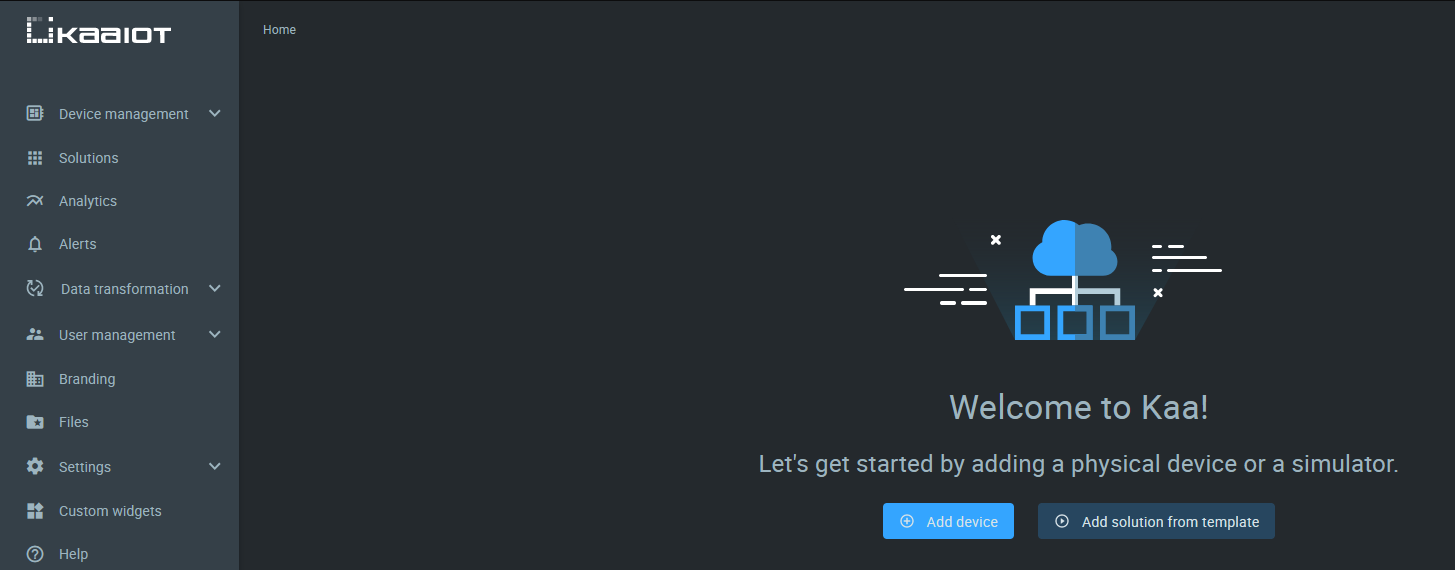
\includegraphics[width=\linewidth]{imagenes/dashboard.png}
    \caption{Dashboard Kaa IoT.}
    \label{fig:figure5}
\end{figure}


\section{Conectar dispositivo}

En este apartado se trata de explicar el proceso de conexión de un dispositivo con nuestra aplicación, desde crear un endpoint hasta ver la información del dispositivo en nuestra interfaz de usuario. Esto engloba varios términos y conceptos que se van a definir a continuación.

\subsection{Términos y conceptos} \label{initial-terms}

\subsubsection{Endpoints}

Los endpoints representan ``el elemento de las cosas`` del IoT. Un endpoint es cualquier dispositivo terminal que se quiera gestionar, en nuestro caso desde Kaa IoT. Un endpoint puede ser un dispositivo físico o una emulación de software del mismo. Todos los datos que llegan a la aplicación están asociados a endpoints. \cite{kaaiotConcepts}

Para ser precisos, un endpoint puede ser una unidad menor que un dispositivo, lo que significa que un dispositivo físico puede incluir múltiples endpoints. Por ejemplo, quieres gestionar un termostato, para que el aire acondicionado se encienda y apague automáticamente a cierta temperatura.

Se puede gestionar el termostato de una de las siguientes maneras:

\begin{itemize}
    \item Toda la unidad del termostato actúa como un endpoint único que intercambia datos con el servidor.
    \item Los componentes del termostato, como los sensores de temperatura y humedad, interruptor de encendido/apagado, actúan como endpoints individuales.
\end{itemize}

\subsubsection{ID de Endpoint}

El ID de endpoints se utiliza para identificar de forma única un endpoint dentro de una instancia. Un ID de endpoints suele ser un UUID generado automáticamente por el framework en el momento de crear un nuevo endpoint. No obstante, también se permiten los ID de endpoints definidos por el usuario. El ID de los endpoints no puede modificarse una vez creado.

Todos los datos de los endpoints, como los atributos de los metadatos, los puntos de datos de series temporales recopilados, los comandos, etc., están asociados a un ID de endpoint específico. Siempre que recupere o gestione datos relacionados con endpoints en Kaa, principalmente a través de la API REST, se verá los ID de endpoints.

\subsubsection{Token del Endpoint} \label{llamada-mqtt}

Los tokens de endpoints se utilizan para la identificación de endpoints cuando se intercambian datos relacionados con los endpoints, utilizando los protocolos compatibles basados en MQTT y HTTP. Los tokens de endpoint son únicos dentro de una aplicación IoT y se asignan exactamente a un endpoint.

Cuando llega un mensaje de un cliente, el token del endpoint se resuelve en el correspondiente ID del endpoint. Un ejemplo sobre el protocolo MQTT, el token del endpoint va dentro de la llamada MQTT, por ejemplo:

\begin{lstlisting}[language=HTML]
kp1/<APPLICATION_VERSION>/epmx/<ENDPOINT_TOKEN>/get
\end{lstlisting}

Normalmente, los tokens son cadenas generadas automáticamente por el framework, pero también se puede crear un token como el usuario quiera, por ejemplo, por el número de serie del dispositivo, dirección MAC, etc.

\subsubsection{Metadatos del endpoint}

Los metadatos de los endpoints son un conjunto de atributos clave-valor asociados a un endpoint. Se representan en el framework como un documento JSON de formato arbitrario.

Los metadatos de endpoints suelen incluir alguna información relacionada con los endpoints, como la ubicación, la descripción, el número de serie, la versión de hardware, etc. Los metadatos se almacenan en el servicio de registro de endpoints y pueden leerse o actualizarse de dos maneras:

\begin{itemize}
    \item A través de la capa de comunicación.
    \item A través de la API REST.
\end{itemize}

También se pueden gestionar los metadatos mediante la interfaz de usuario del framework.

\subsubsection{Aplicaciones y versiones}

Las aplicaciones en Kaa IoT sirven como contenedores para endpoints de diferentes tipos. Se puede tener una aplicación que contenga todos los endpoints que representan a un determinado dispositivo, y una aplicación para otro dispositivo, independiente de la otra aplicación. Las aplicaciones IoT también albergan toda la configuración del sistema necesaria para que el framework conozca las capacidades de sus dispositivos conectados y cómo trabajar con ellos.

Puede pasar que ya hemos configurado nuestro dispositivo, pero queremos implementar una nueva característica. Al implementarla se actualiza el firmware del dispositivo y se empieza a desplegar pero, ¿como diferenciamos entre los dispositivos que ya tienen el nuevo firmware y las que no? Aquí aparecen las versiones de una aplicación.

Cada aplicación puede tener varias versiones al mismo tiempo. Cada versión representa un conjunto de capacidades soportadas por los endpoints. En cualquier momento, cada endpoint está asociado a una versión de su aplicación. El conocimiento de la versión actual de la aplicación de un endpoint ayuda al framework a entender qué funcionalidad soporta el endpoint, cómo se formatean los datos, etc. Se puede utilizar las versiones para hacer evolucionar los dispositivos añadiendo o retirando funcionalidades mientras mantiene sus versiones antiguas en funcionamiento. Para diferenciar llamadas entre versiones se puede indicar como hemos visto en \ref{llamada-mqtt}.

\subsection{Pasos a seguir}

\subsubsection{Crear una aplicación y una versión}

Como hemos visto en \ref{initial-terms}, para registrar un endpoint en nuestro framework necesitamos una aplicación y una versión de esta. Esto podemos gestionarlo desde la interfaz de usuario, concretamente en la sección ``Applications``, una vez en la sección usaremos el botón de ``Add application``. Introduciremos el nombre de la aplicación (campo obligatorio) y tendremos la posibilidad de introducir una descripción. En nuestro caso la aplicación se llamará ``TFG-DASIoT``. \\

Hay que tener en cuenta que tanto las aplicaciones como las versiones tienen:

\begin{itemize}
    \item Nombres autoasignados e inmutables que suelen ser como  \textbf{7bfdd6b9-ff44-4098-a4dc-58c0f3c9f693-v1}. Se utilizarán para las llamadas a la API, la integración con el cliente, etc.
    \item Nombres de visualización arbitrarios que se pueden cambiar en cualquier momento. Estos nombres se utilizan en la interfaz de usuario de la plataforma para una mejor experiencia de usuario. Por ejemplo, en nuestro caso el nombre de la aplicación y la descripción que hayamos puesto.
\end{itemize}

\begin{figure}[hb!]
    \centering
    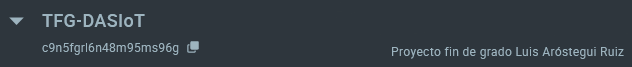
\includegraphics[width=\linewidth]{imagenes/app-creada.png}
    \caption{Nombre y descripción de la aplicación}
    \label{fig:figure6}
\end{figure}

En la imagen también se puede observar como hay un identificador justo debajo del nombre que le hemos asignado a la aplicación, esto es para referenciar de manera univoca a esta. Y ahora que tenemos la aplicación, creamos una versión de esta.

\begin{figure}[ht!]
    \centering
    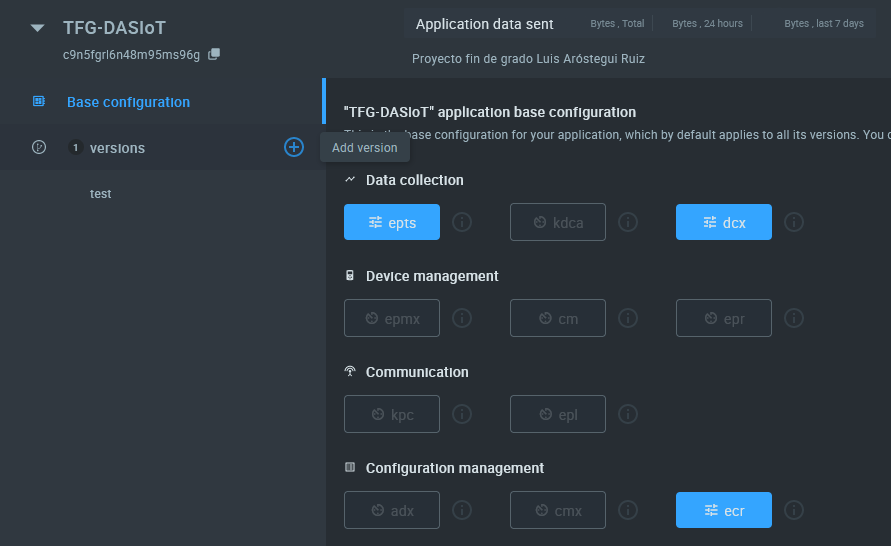
\includegraphics[width=\linewidth]{imagenes/app-version.png}
    \caption{Versiones de la aplicación}
    \label{fig:figure7}
\end{figure}

La primera versión que hemos creado se llama ``test``. Y en la información de la aplicación podemos ver los servicios que tenemos activos.

\begin{itemize}
    \item \textbf{Data collection}. \textit{epts}, se refiere al servicio de series temporales de endpoints. Recibe muestras de datos de endpoints y los transforma en series temporales. \textit{dcx}, es un servicio de recogida de datos, permite a los endpoints enviar muestras de datos de telemetría a la aplicación.
    \item \textbf{Configuration management}. \textit{ecr}, configuración del repositorio del endpoint, almacena los datos de configuración de los endpoints y proporciona una API REST para la gestión.
\end{itemize}

\subsubsection{Crear un endpoint}

En la sección de ``Devices`` de nuestro dashboard, podremos añadir un nuevo dispositivo. Aqui indicaremos, la aplicación a la que va a estar asociada el dispositivo, un nombre para nuestro endpoint y opcionalmente podremos añadir metadatos.

\begin{figure}[p]
    \centering
    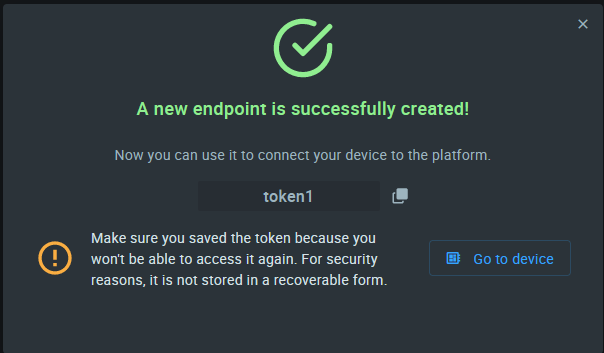
\includegraphics[width=\linewidth]{imagenes/device-added.png}
    \caption{Endpoint creado}
    \label{fig:figure8}
\end{figure}

\begin{figure}[p]
    \centering
    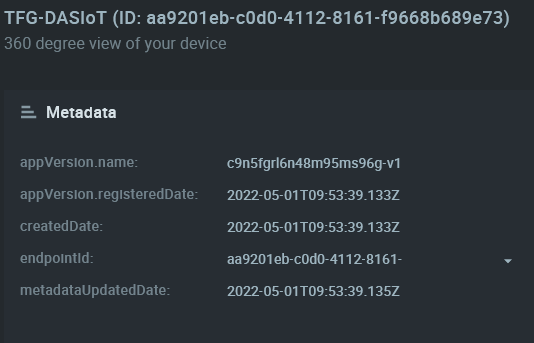
\includegraphics[width=\linewidth]{imagenes/device-created-view.png}
    \caption{Datos del dispositivo creado}
    \label{fig:figure9}
\end{figure}

En nuestro caso, para referirnos al endpoint lo hacemos mediante el \textit{token endpoint} \ref{llamada-mqtt}, que como vemos en \ref{fig:figure8}, se llama token1. Esto lo usaremos en nuestra llamada mqtt para hacer referencia a este dispositivo.\\

Para ver todos los datos del dispositivo se nos muestra como vemos en \ref{fig:figure9}. Donde podemos ver la aplicación a la que esta asociada, la fecha de creación y de su última actualización.

\newpage

\subsubsection{Conectar un cliente}

Una vez ya hemos creado nuestro primer endpoint, podemos conectar un cliente y obtener y enviar algunos metadatos. Como se analizó \ref{eleccion-framework}, Kaa IoT es un framework que soporta varios protocolos donde nos encontramos con HTTP y MQTT \ref{protocolos}.

Para hacer uso de los protocolos y completar la integración del cliente necesitaremos el nombre de la versión y el token del endpoint. En esta sección se va a mostrar como hacer uso de ambos protocolos, concretamente de las órdenes para poder ejecutar la conexión con nuestro dispositivo, en la sección de \textit{Pruebas} \ref{pruebas} se mostrarán los datos que obtenemos tras su ejecución.\\

\paragraph{Conexión mediante HTTP}

Para obtener todos los atributos de los metadatos con \textbf{HTTP} vamos a hacer uso de cURL \footnote{Es un proyecto de software consistente en una biblioteca y un intérprete de comandos orientado a la transferencia de archivos. Soporta los protocolos FTP, FTPS, HTTP, HTTPS, TFTP, SCP, SFTP, Telnet, DICT, FILE y LDAP, entre otros.} para enviar una solicitud de actualización de datos del dispositivo.

\begin{lstlisting}[language=bash]
curl - -location - -request POST 'https://connect.cloud.kaaiot.com:443/kp1/
<app-version-name>/epmx/<endpoint-token>/update/keys' \
- -data-raw '{
    "model": "BFG 9000",
    "mac": "00-14-22-01-23-45"
}'
\end{lstlisting}

Ejecutando esta instrucción añadiremos nuevos metadatos a nuestro dispositivo, concretamente la dirección física y el modelo de este.

\paragraph{Conexión mediante MQTT}

Para hacer la conexión mediante \textbf{MQTT} se ha optado por la opción de usar Python en su versión 3.10, obtenemos un código como el siguiente.

\begin{lstlisting}[language=Python]
import itertools
import json
import queue
import random
import string
import sys
import time

import paho.mqtt.client as mqtt
from decouple import config

KPC_HOST = config('KPC_HOST', cast=str)
KPC_PORT = config('KPC_PORT', cast=int)

APPLICATION_VERSION = config('APPLICATION_VERSION', cast=str)
ENDPOINT_TOKEN = config('ENDPOINT_TOKEN', cast=str)


class MetadataClient:

    def __init__(self, client):
        self.client = client
        self.metadata_by_request_id = {}
        self.global_request_id = itertools.count()
        get_metadata_subscribe_topic = f'kp1/{APPLICATION_VERSION}/epmx/{ENDPOINT_TOKEN}/get/#'
        self.client.message_callback_add(get_metadata_subscribe_topic, self.handle_metadata)

    def handle_metadata(self, client, userdata, message):
        request_id = int(message.topic.split('/')[-2])
        if message.topic.split('/')[-1] == 'status' and request_id in self.metadata_by_request_id:
            print(f'<--- Received metadata response on topic {message.topic}')
            metadata_queue = self.metadata_by_request_id[request_id]
            metadata_queue.put_nowait(message.payload)
        else:
            print(
                f'<--- Received bad metadata response on topic {message.topic}:\n{str(message.payload.decode("utf-8"))}')

    def get_metadata(self):
        request_id = next(self.global_request_id)
        get_metadata_publish_topic = f'kp1/{APPLICATION_VERSION}/epmx/{ENDPOINT_TOKEN}/get/{request_id}'

        metadata_queue = queue.Queue()
        self.metadata_by_request_id[request_id] = metadata_queue

        print(f'---> Requesting metadata by topic {get_metadata_publish_topic}')
        self.client.publish(topic=get_metadata_publish_topic, payload=json.dumps({}))
        try:
            metadata = metadata_queue.get(True, 5)
            del self.metadata_by_request_id[request_id]
            return str(metadata.decode("utf-8"))
        except queue.Empty:
            print('Timed out waiting for metadata response from server')
            sys.exit()

    def patch_metadata_unconfirmed(self, metadata):
        partial_metadata_udpate_publish_topic = f'kp1/{APPLICATION_VERSION}/epmx/{ENDPOINT_TOKEN}/update/keys'

        print(f'---> Reporting metadata on topic {partial_metadata_udpate_publish_topic}\nwith payload {metadata}')
        self.client.publish(topic=partial_metadata_udpate_publish_topic, payload=metadata)


def main():
    # Inicializar conexion con el servidor
    print(
        f'Connecting to Kaa server at {KPC_HOST}:{KPC_PORT} using application version {APPLICATION_VERSION} and endpoint token {ENDPOINT_TOKEN}')

    client_id = ''.join(random.choice(string.ascii_uppercase + string.digits) for _ in range(6))
    client = mqtt.Client(client_id=client_id)
    client.connect(KPC_HOST, KPC_PORT, 60)
    client.loop_start()

    metadata_client = MetadataClient(client)

    # Obtener los atributos de los metadatos del endpoint actual
    retrieved_metadata = metadata_client.get_metadata()
    print(f'Retrieved metadata from server: {retrieved_metadata}')

    # Actualizar parcialmente los metadatos del endpoint
    metadata_to_report = json.dumps({"model": "BFG 9001", "mac": "00-14-22-02-23-45"})
    metadata_client.patch_metadata_unconfirmed(metadata_to_report)

    time.sleep(5)
    client.disconnect()


if __name__ == '__main__':
    main()

\end{lstlisting}

La ejecución de este código produce el mismo efecto que el visto con HTTP. Se usa \textit{decouple} para evitar mostrar los datos de configuración de la aplicación, como el endpoint o la versión de la aplicación (lineas 12-16).
}

\section{Recogida de datos de un dispositivo}